\newpage
\chapter{Conclusion and Discussion}\label{discussion}

% This project has shown that both mutation location in the genome and the composition of mutations were important characteristics of the cancer mutation profile. Regarding the genomic location effect (GLE), mutations were shown to preferably occur in closed chromatin regions over open chromatin regions. GLE helped characterise the mutation profile because it differed significantly between cancers. More importantly, the smooth representation was better at extracting information from GLE than the bin representation for cancer classification (Chapter \ref{gle}). Regarding the sequence context (SCE) for mutation composition, this project has shown that SCE contributes a considerable amount of information to the cancer mutation profile. Cancers had very different composition of mutations and the difference came from both the base substitutions and the flanking bases. Mutation composition was strand-symmetric and there was more information from transitions than there was from transversions (Chapter \ref{sce}). The project also developed a mutation-based classifier of cancer using the distance-based algorithm KNN. In general, I found that both GLE and SCE were shown to be predictive of cancers but SCE was the dominating predictor (Chapter \ref{ml}). 

% Sections \ref{discussion:gle} and \ref{discussion:sce} of this chapter discusses the properties of the GLE and SCE via both the results from statistical analyses of whole diseases and the representations from the classifier training. Section \ref{discussion:miclassification} speculates the reasons behind certain patterns of misclassification and proposes ways to improve accuracy in future projects. Section \ref{discussion:diagnosis} describes the potential advantages of developing mutation-based classifiers in the long term.

\section{Genomic location effect}\label{discussion:gle}
\subsection{Speculation of the mechanisms driving GLE}
% My conclusion that mutations tend to occur in closed regions agree with previous observations \citep{Polak2015,Fujimoto2016Whole-genomeCancer,Prendergast2007ChromatinGenome}. Notably, \citet{Polak2015} used different measures of chromatin structure, including DHS and histone marks such as H3K4me1, to predict mutation density in Mbp bins. The $OR$ mislabelling experiment of this project found that chromatin structure of the original cells was influential on GLE but unlikely to determine whether GLE differed between cancers (Section \ref{gle:mixed_or}) whereas \citet{Polak2015} showed that chromatin structure data from the correct cell types of origin were more correlated with the mutation density of the cancer than mislabelled cell types. The two results were not directly compatible, as the difference might have come from the different set of cancers investigated and the different types of data representing chromatin status (explained below). However, looking at the reported variance explained $R^2$ from \citet{Polak2015}, their claim was only really convincing for skin melanoma (Skin-Melanoma) and hepatocellular carcinoma (Liver-HCC), two distinct cancers even in my project. 

% Several factors could potentially interfere with the reliability of the DHS data recruited to represent chromatin status. First, for simplicity, I used the binary representation of DHS that treats genomic regions as either open or closed regions. However, the accessibility of DNA is actually more complicated, as there is variation in the openness of open chromatin regions \citep{Boyle2008High-ResolutionGenome}. A continuous representation instead of the binary representation used in this project would therefore be more accurate. Second, there was a degree of uncertainty in the identification of the cells of origin. This is particularly true for medulloblastoma (CNS-Medullo), whose cell types of origin is still just a speculation \citep{Penas2015TheMedulloblastoma} but less true in skin melanoma, whose original cell type is quite established to be melanocyte \citep{Lin2007MelanocytePigmentation}. Besides, each DHS data for a cell type provided by ENCODE came from only one individual, but variation among individuals is quite likely \citep{Thurman2012TheGenome}. Third, chromatin structure could be modified during carcinogenesis, for example due to mutations in chromatin modifier genes \citep{Makova2015TheGenome}. While this is an identified problem, there is no easy way to account for it given the availability of accessible data that I am aware of. I expect that using DHS data for the cancer itself rather than its original cell type is unlikely the solution because the modifications in chromatin structure differ between samples of similar cancer type across different stages of cancer. 

% Assuming DHS data is reliable, I hypothesise another explanation for the ability of GLE to predict cancers: the interaction between chromatin structure and the distribution of base compositions across the genome rather than the chromatin structure itself. This is explained in Figure \ref{fig:discussion_gle}. Essentially, I hypothesise that some genomic regions have higher mutation density not only because they are in the closed chromatin but also because they contain bases that are prone to be targeted by a specific mutagen. Given that chromatin structure affects GLE, this explanation will make sense if the variation in chromatin structure is not great enough to shape the diversity of GLE \textit{per se}. Indeed, \citet{Gilbert2004ChromatinFibers} showed that open chromatin regions contain gene clusters, hypothetically for expression and protection of genes \citep{Gilbert2004ChromatinFibers,Gazave2005DoesDamage}. This suggests a certain degree of conservativeness in chromatin structure as genes universal to all cell types will be more likely located in open chromatin regions. My proposed explanation can be evaluated by examining the association between the types of substitutions (whether the wildtype is A/T or C/G) and their location (whether they locate in closed or open chromatin regions) as well the association between the cancer type (whether mutations with wildtype A/T are from cancer A or B) and their genomic location with respect to the cancers (closed or open regions). The statistical techniques for the suggested analyses are similar to the G-test and $OR$ described in Methods \ref{methods:chromatin}, but the tables involved should be similar to those presented in Figure \ref{fig:discussion_gle}.

\begin{figure}[h!]
  \begin{minipage}[c]{\textwidth}
    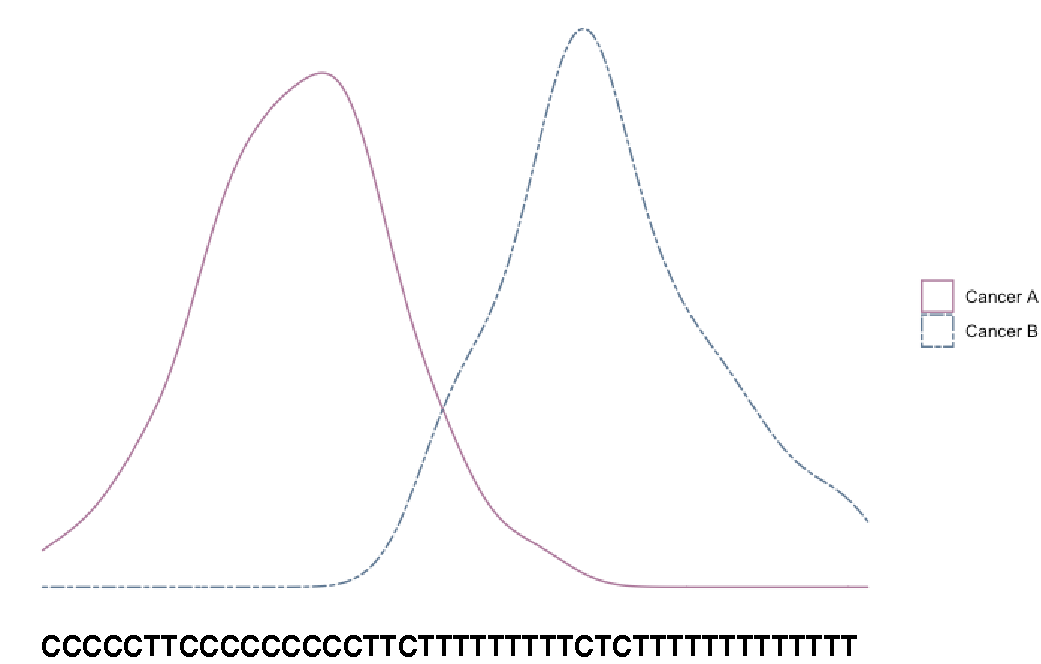
\includegraphics[scale=0.9]{graphics/discussion_gle.pdf}
  \end{minipage}\hfill
  \vspace{1cm}
  
  \begin{minipage}[c]{0.48\textwidth}
  \centering
    \begin{tabulary}{\columnwidth}{rRR}
    \toprule
        & \textbf{A/T mutated (Cancer A)} &  \textbf{C/G mutated (Cancer A)} \\
    \hline
        \textbf{closed} &  &   \\
        \textbf{open} &  &   \\
    \bottomrule
    \end{tabulary}
  \end{minipage}\hfill
  \begin{minipage}[c]{0.48\textwidth}
    \begin{tabulary}{\columnwidth}{rRR}
    \toprule
        & \textbf{A/T mutated (Cancer A)} &  \textbf{A/T mutated (Cancer B)} \\
    \hline
        \textbf{closed} &  &   \\
        \textbf{open} &  &   \\
    \bottomrule
    \end{tabulary}
  \end{minipage}
  \vspace{0.5cm}
  
  \begin{minipage}[c]{\textwidth}
    \caption{
      \textbf{Proposed explanation for why GLE differ between Cancer A and Cancer B.} Cancer A is under the influence of a mutagen that targets the base C; Cancer B is under the influence of a mutagen that targets the base T. Some regions of the genome are more enriched in C, other are enriched in T. The distribution of bases combines with chromatin structure to influence GLE. This could be evaluated by assessing whether certain substitutions are enriched in closed/open chromatin regions, or whether two cancers differ in how mutations with wildtype A/T are distributed between closed/open chromatin regions.
    } \label{fig:discussion_gle}
  \end{minipage}
\end{figure}


\subsection{Representing GLE}
% In this work, I showed that the smooth representation of GLE was better than the bin representation for both the bootstrap hypothesis testing (Section \ref{gle:bootstrap}) and the GLE-based classification (Section \ref{ml:gle}). For the bootstrap study, the p-value was not necessarily contrasted against a significance threshold, but it really was an indication of the ``extremity'' of the observed distance between cancers. Interestingly, the Wasserstein distance somehow redeemed the performance of the bin representation compared to the smooth representation. As previously mentioned (Figure \ref{fig:mutdistribution_demo} of Section \ref{intro:gle}), the drawback of the bin representation is that it imposes arbitrary rigid boundaries to the genome. However, looking at its definition (Methods Figure \ref{fig:wasserstein_demo}), the Wasserstein allows comparisons of bins with different coordinates, thereby ``breaking'' the rigid boundaries. In other words, the Wasserstein distance itself has a smoothing effect. Regarding the 1 Mbp bin size, \citet{Hodgkinson2012TheGenomes} stated that the variation in GLE was detected at the 1 Mbp scale, but blurred out at the 10 Mbp scale. Although the two scales are quite different, and the Mbp scale was not demonstrated to be the lower limit, at this point we accept that the use of 1 Mbp was reasonable. Accordingly, the choice of using the smooth representation or the bin representation combined with Wasserstein distance should therefore depend on computing performance. 

\section{Sequence context effect}\label{discussion:sce}
\subsection{Patterns of mutation composition}
% Using the measure of information $RE$, I detected patterns of mutation composition that were compatible with previous work \citep[Chapter \ref{sce};][]{Alexandrov2020}. In particular, \citet{Alexandrov2020} decomposed the composition of mutations using non-negative matrix factorisation to identify the so-called ``mutation signatures''. They found that signature SBS7a was found in all skin melanoma samples and was only found in skin melanoma. This signature is predominated by the C$\rightarrow$T substitution, especially when there is a T at flanking position -1. This mutation had previously been established to be associated with the pyrimidine dimer formation between T (position -1) and C (position 0) in combination with the repair systems due to UV light exposure in Skin-Melanoma \citep{Pfeifer2005MutationsLight}. This is consistent with my observation in Figures \ref{fig:spectra_skin} and \ref{fig:transitions_skin}. Likewise, signature SBS12 was detected only in hepatocellular carcinoma was enriched in the A$\rightarrow$G/T$\rightarrow$C substitution, which is in line with the observation in Figure \ref{fig:spectra_liver}. The work of \citet{Alexandrov2020} was a detailed decomposition of mutation compositions, where each cancer could have multiple signatures. In the meantime, my work, developed on top of \citet{Zhu2017}, was analogical to a general summary of mutation composition. 

\subsection{Strand symmetry}
% Both $RE$ (Chapter \ref{sce}) and the SCE-based classifier (Section \ref{ml:sce}) of my project showed evidence of strand symmetry, in the sense that reverse complementary mutations are counted as the same category (introduced in Figure \ref{fig:motif_symmetric_demo} of Section \ref{intro:sce}). This representation, which I referred to as semi-symmetry, was adopted by most publications that I am aware of \citep{Alexandrov2020,Jiao2020,Zhang2020}. However, \citet{Zhu2017} showed that the compositions of flanking bases to a substitution significantly differed between two DNA strands in skin melanoma. This is not necessarily contradictory with my finding, but it reflects the fact that the data I used did not specify what mutations occurred on which DNA strand. Nevertheless, this shows that given this type of data, which is often the case, the semi-symmetry representation should be sufficient to capture information.

\subsection{Flanking bases beyond 3-mers}
% There was inconsistency in the $RE$ of flanking positions (Section \ref{sce:nbr}) and the SCE-based classifier (Section \ref{ml:sce}) with respect to the importance of bases at positions -2 and +2. Even though information was observed in these positions using $RE$, incorporating them into the classifier (5-mer) led to a drop in accuracy. I attributed this to the size of the vector representing 5-mers. Both the attempt to break the 5-mer vector down into shorter vectors (Figure \ref{fig:f1_sce_submotif}) and the introduction of semi-symmetry (Figure \ref{fig:f1_sce}) improved the accuracy over the whole 5-mer vector, which supports my speculation. It is worth noting that the fully symmetric representation worsened the accuracy instead of improving it. This representation was an attempt to shorten the SCE vector without a biological basis; therefore, its results indicate that the length of the representation vector was not a determinant of accuracy without a good biological rationale. In comparison with the literature, \citet{Zhu2020} showed that it was possible to identify the origin of a single mutation based on its flanking bases. \citep{Zhang2020} showed that using the sequence context of the 9-mer context was the best at predicting cancers, both for simulated data and for four breast cancer subtypes. Their results were obtained using the support vector machines, which is a kernel based classifier algorithm \citep{Susmita2019AAlgorithms}. As described in Methods \ref{methods:ml_both}, one way to compute the pairwise kernel matrices is via the pairwise distance matrices.  This is a great support for the potential of incorporating bases beyond 3-mers. However, while \citet{Zhang2020} also split up large context sizes, their representation forced bases of the same distance to the substitution (\textit{e.g.} positions -1 and +1) to have the same weight, which, I suspect, is one of their drawbacks. As previously seen from Figure \ref{sce:nbr}, for a mutation (\textit{e.g.} C$\rightarrow$T), the contribution of position +1 to the information context was different from that of position -1, unlike the assumption in \citet{Zhang2020}. While \citet{Zhang2020} reported a context size of 9-mer for the data they had (simulated data and breast cancers), two questions worth examining in future project concerns (1) what is the maximum size of sequence context in which the furthest flanking bases from the substitution are still informative and (2) whether this sequence context size is uniform between cancers. 

\section{Misclassification and improvement of accuracy}\label{discussion:miclassification}
\subsection{Common patterns of misclassification}
% Some patterns of misclassification can be observed for the GLE-based classifiers, but there was no obvious patterns for the SCE-based classifiers. Prior to the project, I had expected the GLE-based classifiers to misclassify epigenetically similar cancers due to the influence of chromatin structures on GLE. However, it is important to note that epigenetically similar cells are also likely to be under the influence of chemically similar environments (\textit{e.g.} similar mutagens). This expectation was true for the two lymphocyte related cancers, chronic lymphocytic leukaemia (Lymph-CLL) and B-cell non-Hodgkin's lymphoma for all representations and distance measures (Figures \ref{fig:confusion_smooth_euclidean}, \ref{fig:confusion_bin_euclidean} and \ref{fig:apdx_ml_gle}). From the multidimensional scaling plot (Figure \ref{fig:encode_pca}), which groups epigenetically similar cell types together, because Skin-Melanoma and Liver-HCC were far away from other cancers, they were expected to be distinctive cancers. This was generally the case, with the exception of the bin representation using the Euclidean distance. Almost all donors with Skin-Melanoma and Liver-HCC were correctly identified, and donors predicted to have these cancers really did. From Figure \ref{fig:encode_pca}, we would expect prostate adenocarcinoma (Prost-AdenoCA) and pancreatic adenocarcinoma (Panc-AdenoCA) to be misclassified because they seemed very similar in terms of chromatin structure. This expectation was only partly met when using the Wasserstein distance (Figure \ref{fig:apdx_ml_gle}). Regarding the SCE-based classifiers, the misclassified cancers were not consistent between different representations. One vague pattern was that CNS-Medullo was sometimes mistaken for Prost-AdenoCA (for the 3-mer and the submotif classifiers, Figures \ref{fig:confusion_3mer}, \ref{fig:confusion_3mer_symmetric}, \ref{fig:confusion_2-submotifs} and \ref{fig:confusion_3-submotifs}). At this point, it is uncertain whether this suggests some interesting common patterns of mutation compositions between the two cancers or just an artefact. 

% In comparison with the previous study by \citet{Jiao2020}, it was also found that misclassification was common between Lymph-CLL and Lymph-BNHL and between the brain cancers CNS-Medullo and pilocytic astrocytoma (CNS-PiloAstro). The former was consistent but the latter was not observed for our project. \citet{Jiao2020} attributed the misclassification patterns to the similarity in the epigenetics of the cancers. Based on my analysis of the chromatin structure, I only partly agree with this speculation. I propose that chromatin structure has some contribution to the misclassification but there are other parallel factors involved. An example of such factors is illustrated in Figure \ref{fig:discussion_gle}.

\subsection{Classification accuracy}
% The best performing classifier for GLE was the smooth representation using Euclidean distance (mean $F1=0.59$; Section \ref{ml:gle}); the best performing classifier for SCE was the 3-mer representation (mean $F1=0.83$; Section \ref{ml:sce}). Combining GLE and SCE did not improve accuracy; instead, the accuracy was mostly determined by SCE (Section \ref{ml:both}). \citet{Jiao2020} also attempted to develop classifiers of cancers based on mutation data. Using the Random Forest (RF) classifier algorithm \citep{Lindner2017AutomatedModels}, they found that the classifiers by either GLE or SCE individually produced $F1\approx0.7$. Their attempt to combine GLE, SCE and other factors (such as the genomic distribution of copy number variations or structural variation) resulted in a median $F1=0.86$. Because GLE and SCE were the most accurate in their examined predictors, it can be assumed that $F1=0.86$ was mostly contributed by the two factors. The improvement of accuracy when combining GLE and SCE over the individual classifiers in the case of \citet{Jiao2020} might be because their individual classifiers were compatible with respect to accuracy. In the meantime, the level of accuracy for the joint classifier in my case only depended on SCE, possibly because my SCE-based classifier was much more accurate than the GLE-based classifier in the first place. 

\subsubsection{Improving accuracy by data representations}
% There are several tweaks to the representation of both GLE and SCE that could potentially improve accuracy over the models developed during my project. For GLE, I have computed the distances between donors by summing up the distances for all chromosomes. Knowing that chromosomes vary in lengths, we could try weighing different chromosomes according to their lengths. For SCE, because the evidence supporting the usefulness of flanking bases beyond 3-mers was plenty, including the measure of information in Section \ref{sce:nbr} and the results reported by \citet{Zhang2020}, further effort should focus on incorporating larger $k$-mer sizes. We have seen that information was available in positions -2 and +2, but less than that in positions -1 and +1 (Section \ref{sce:nbr}). In this project, I gave all flanking positions the same weights. In future project, we could experiment with imposing weights on different components of the submotif representation for SCE. Finally, based on the speculation in Figure \ref{fig:discussion_gle}, it is also worth considering a way to represent the interaction between GLE and SCE. This could be in the form of an interaction term between the two factors, or a single factor that simultaneously accounts for both factors.

\subsubsection{Addressing imbalanced data}
% One issue that has not been addressed in my project and \citet{Jiao2020} is the imbalanced data for classification. In my project, some cancers had more than 200 donors (\textit{e.g.} Liver-HCC) and some only had fewer than 80 donors (\textit{e.g.} bone osteosarcoma, Bone-Osteosarc). This could lead to biased predictions, described in Figure \ref{fig:imbalanced}, in which new observations of the minor class are misclassified as the major class because there are not enough data points supporting the minor in the training set. For my project, this was most obvious in Bone-Osteosarc (44 donors), which tended to be identified as another cancer in a seemingly random manner. Established techniques to address the issue of imbalanced classification worth taken into consideration include under-sampling and over-sampling. Both techniques attempt to make the number of data points roughly similar between the major and the minor class. Under-sampling involved excluding data from the major class and keeping the number of data points from the minor class, which is quite straightforward \citep{Kubat1997AddressingSelection}. Over-sampling involved simulating more data from the minor class and keeping the number of data points from the major class \citep{Chawla2002SMOTE:Technique}. Specifically, the over-sampling simulation introduced by \citet{Chawla2002SMOTE:Technique} is a distance-based algorithm that creates new observations that are closer to the minor class than the major class. 

\begin{figure}[ht!]
    \centering
    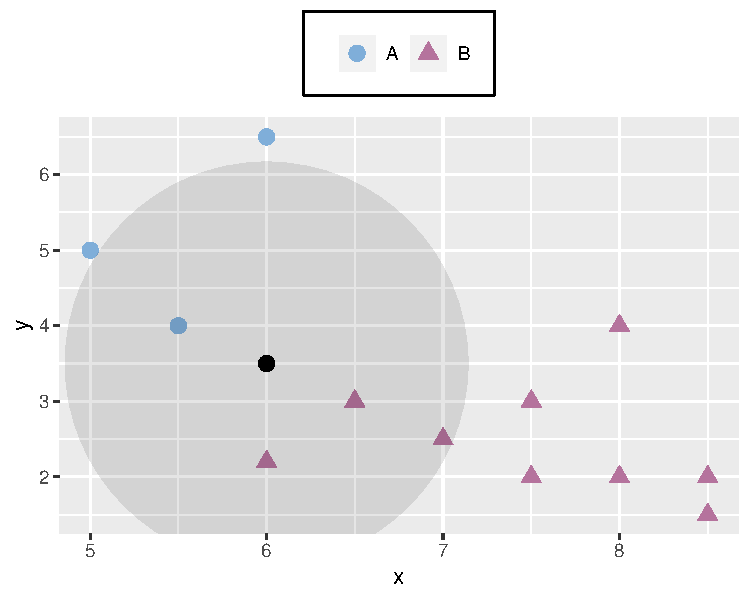
\includegraphics[scale=0.9]{graphics/imbalanced.pdf}
    \caption{\textbf{Impact of imbalanced design.} Cancer A (circle) is the minor cancer with fewer observations. Cancer B (triangle) is the major cancer with more observations. When a new data point representing Cancer A (black circle) is to be predicted, it tends to be misclassified as Cancer B because there is not enough confidence for the classifier to predict it to be Cancer A.}
    \label{fig:imbalanced}
\end{figure}


\subsubsection{Choosing the machine learning algorithms}
% The choice of the machine learning algorithms could also affect accuracy. For example, when training a classifier combining GLE and SCE, \citet{Jiao2020} reported that the deep neural network (DNN) classifier was better than the RF classifier (DNN was not used to train GLE and SCE individually). Even though there are known strengths and drawbacks for each classifier \citep{Susmita2019AAlgorithms}, which algorithm is the most accurate can be very context dependent. In this project, I chose the KNN because it was convenient for my distance-based representation of data and because of its interpretability. By contrast, DNN is often thought of as a ``black box'' that is hard to understand and manipulate \citep{Shwartz-Ziv2017OpeningInformation}. However, in future work, it is worth experimenting with different algorithms and establishing which algorithms are suitable for mutation-based classifiers of cancers. 

\section{Cancer diagnosis and mutation based classifiers}\label{discussion:diagnosis}
% Cancer diagnosis is an important step in cancer management \citep{Tobias2014CancerManagement}. Early diagnosis is one of the keys to cancer treatment \citep{Hawkes2019CancerDiagnosis}. For this reason, several schemes for cancer screening have been employed to detect certain cancers in high risk individuals on a population scale \citep{Tobias2014CancerManagement}. For example, women aged 20-65 in the UK are encouraged to have a Papanicolaou test \citep{Bharadwaj2013HumanTreatment} to screen for cervical cancers every three years \citep{Tobias2014CancerManagement}. It would be beneficial to be able to detect cancers systematically at an early stage. As mentioned in Section \ref{intro:significance}, with the development of liquid biopsy, it might be possible in the long term that we could predict what cancer is present based on circulating tumour DNA in the blood upon successful development of a mutation-based classifier. In terms of diagnosis, multiple evaluations are usually required to reach a conclusion \citep{Tobias2014CancerManagement,Stone1995Biopsy:Pitfalls}. Two important tools for cancer diagnosis are biopsy and immunohistochemistry (IHC), which require manual interpretation of trained pathologists \citep{Stone1995Biopsy:Pitfalls,Ahmed200615Cancer}. However, it can sometimes be challenging even for trained pathologists to correctly identify cancers from IHC without prior knowledge of other factors such as the patients' clinical history, particularly when given a \gls{metastasis} of unknown primary \citep{Sheahan1993MetastaticStatus,Rassy2020ExploringToday}.  

% As a result, it is always desirable to have an additional diagnostic tool, particularly a quantitative one with explicit numeric measures of prediction confidence. Whilst there is a long way to go, my project is a demonstration of the feasibility of such a tool. The classifiers trained in this project were completely based on mutation data. Both aspects of the mutation profile examined were backed up by statistical analyses. The performance of the classifiers I developed was certainly better than random prediction (a rough estimation of the random threshold in this case is an accuracy score $<\frac{1}{12}$ because 12 cancers were analysed). If such a classifier is successfully developed in real life, it can act as either an exploratory evaluation or a validation tool for cancer diagnosis because it approaches the problem from a different perspective to a pathologist's. 

\section{Concluding remarks and summary of the future directions}\label{discussion:conclusion}
% Mutation patterns are very distinct for different cancers, hypothetically because they inherit some characteristics of the environments in their original cells. Using statistical tools, my project explored the information content available in two aspects of cancer mutagenesis: the location of mutations (GLE) and the composition of somatic point mutations (SCE). First, I found that GLE was influenced by chromatin status but the distinctness of GLE in different cancers was unlikely to come from chromatin structure. I confirmed that there was a ``distortion'' of data when imposing arbitrary boundaries to the genome via the bin representation, which can be compensated for by a distance measure that are not strictly point-wise like the Wasserstein. Second, I found that reverse complementary elements of mutations were strand symmetric and that transitions were typically more informative than transversions. I found that information was available in positions -2 and +2, though less than in positions -1 and +1. However, extracting this information was not easy due to the rapidly increasing size of the SCE vector when incorporating more flanking positions.

% In future projects, it would be desirable to gain more understanding of the sequence context size affecting SCE as well as the interaction between SCE and GLE. To improve accuracy, we should try assigning weights to different components of the representation vectors (chromosomes for GLE; flanking bases for SCE). In addition, creating balanced data before classification and using different machine learning algorithms are also worth trying.